\section{Data}
\subsection{Linked Census Microdata}\label{sec:data-IPUMS}

I collect economic and demographic data on the populations of interest 
from the full count decennial censuses taken in 1940 and 1950
\citep{rugglesIPUMSAncestryFull2024}.
IPUMS also provides linked individual census data up until 1950
through their Multigenerational Longitudinal Panel (MLP) project
\citep{rugglesIPUMSMultigenerationalLongitudinal2025}.
I use the links between the 1940 and 1950 full-count censuses
from version 2.0 of the MLP data provided by IPUMS.
For my main analysis sample,
I select all individuals 
whose reported race in 1940 was either Japanese or Chinese,
who born before 1926 (so that they would have been of working age by World War II),
and who are not missing income or employment data in either census.
This leaves me with a linked sample of 8,136 individuals,
of which about three quarters of whom are Japanese
and one quarter are Chinese.

\begin{table}
  \caption{\label{tbl:mlp_sumstats}Summary statistics for Chinese and Japanese linked in MLP}
  \begin{adjustbox}{width=.9\textwidth, center}
\begin{tblr}[         %% tabularray outer open
]                     %% tabularray outer close
{                     %% tabularray inner open
colspec={Q[]Q[]Q[]Q[]Q[]Q[]Q[]},
cell{2}{1}={}{halign=l,},
cell{3}{1}={}{halign=l,},
cell{4}{1}={}{halign=l,},
cell{5}{1}={}{halign=l,},
cell{6}{1}={}{halign=l,},
cell{7}{1}={}{halign=l,},
cell{8}{1}={}{halign=l,},
cell{9}{1}={}{halign=l,},
cell{10}{1}={}{halign=l,},
cell{11}{1}={}{halign=l,},
cell{12}{1}={}{halign=l,},
cell{13}{1}={}{halign=l,},
cell{14}{1}={}{halign=l,},
cell{15}{1}={}{halign=l,},
cell{16}{1}={}{halign=l,},
cell{17}{1}={}{halign=l,},
cell{18}{1}={}{halign=l,},
cell{19}{1}={}{halign=l,},
cell{1}{1}={}{halign=l, halign=c,},
cell{2}{2}={}{halign=r,},
cell{2}{3}={}{halign=r,},
cell{2}{4}={}{halign=r,},
cell{2}{5}={}{halign=r,},
cell{2}{6}={}{halign=r,},
cell{2}{7}={}{halign=r,},
cell{3}{2}={}{halign=r,},
cell{3}{3}={}{halign=r,},
cell{3}{4}={}{halign=r,},
cell{3}{5}={}{halign=r,},
cell{3}{6}={}{halign=r,},
cell{3}{7}={}{halign=r,},
cell{4}{2}={}{halign=r,},
cell{4}{3}={}{halign=r,},
cell{4}{4}={}{halign=r,},
cell{4}{5}={}{halign=r,},
cell{4}{6}={}{halign=r,},
cell{4}{7}={}{halign=r,},
cell{5}{2}={}{halign=r,},
cell{5}{3}={}{halign=r,},
cell{5}{4}={}{halign=r,},
cell{5}{5}={}{halign=r,},
cell{5}{6}={}{halign=r,},
cell{5}{7}={}{halign=r,},
cell{6}{2}={}{halign=r,},
cell{6}{3}={}{halign=r,},
cell{6}{4}={}{halign=r,},
cell{6}{5}={}{halign=r,},
cell{6}{6}={}{halign=r,},
cell{6}{7}={}{halign=r,},
cell{7}{2}={}{halign=r,},
cell{7}{3}={}{halign=r,},
cell{7}{4}={}{halign=r,},
cell{7}{5}={}{halign=r,},
cell{7}{6}={}{halign=r,},
cell{7}{7}={}{halign=r,},
cell{8}{2}={}{halign=r,},
cell{8}{3}={}{halign=r,},
cell{8}{4}={}{halign=r,},
cell{8}{5}={}{halign=r,},
cell{8}{6}={}{halign=r,},
cell{8}{7}={}{halign=r,},
cell{9}{2}={}{halign=r,},
cell{9}{3}={}{halign=r,},
cell{9}{4}={}{halign=r,},
cell{9}{5}={}{halign=r,},
cell{9}{6}={}{halign=r,},
cell{9}{7}={}{halign=r,},
cell{10}{2}={}{halign=r,},
cell{10}{3}={}{halign=r,},
cell{10}{4}={}{halign=r,},
cell{10}{5}={}{halign=r,},
cell{10}{6}={}{halign=r,},
cell{10}{7}={}{halign=r,},
cell{11}{2}={}{halign=r,},
cell{11}{3}={}{halign=r,},
cell{11}{4}={}{halign=r,},
cell{11}{5}={}{halign=r,},
cell{11}{6}={}{halign=r,},
cell{11}{7}={}{halign=r,},
cell{12}{2}={}{halign=r,},
cell{12}{3}={}{halign=r,},
cell{12}{4}={}{halign=r,},
cell{12}{5}={}{halign=r,},
cell{12}{6}={}{halign=r,},
cell{12}{7}={}{halign=r,},
cell{13}{2}={}{halign=r,},
cell{13}{3}={}{halign=r,},
cell{13}{4}={}{halign=r,},
cell{13}{5}={}{halign=r,},
cell{13}{6}={}{halign=r,},
cell{13}{7}={}{halign=r,},
cell{14}{2}={}{halign=r,},
cell{14}{3}={}{halign=r,},
cell{14}{4}={}{halign=r,},
cell{14}{5}={}{halign=r,},
cell{14}{6}={}{halign=r,},
cell{14}{7}={}{halign=r,},
cell{15}{2}={}{halign=r,},
cell{15}{3}={}{halign=r,},
cell{15}{4}={}{halign=r,},
cell{15}{5}={}{halign=r,},
cell{15}{6}={}{halign=r,},
cell{15}{7}={}{halign=r,},
cell{16}{2}={}{halign=r,},
cell{16}{3}={}{halign=r,},
cell{16}{4}={}{halign=r,},
cell{16}{5}={}{halign=r,},
cell{16}{6}={}{halign=r,},
cell{16}{7}={}{halign=r,},
cell{17}{2}={}{halign=r,},
cell{17}{3}={}{halign=r,},
cell{17}{4}={}{halign=r,},
cell{17}{5}={}{halign=r,},
cell{17}{6}={}{halign=r,},
cell{17}{7}={}{halign=r,},
cell{18}{2}={}{halign=r,},
cell{18}{3}={}{halign=r,},
cell{18}{4}={}{halign=r,},
cell{18}{5}={}{halign=r,},
cell{18}{6}={}{halign=r,},
cell{18}{7}={}{halign=r,},
cell{19}{2}={}{halign=r,},
cell{19}{3}={}{halign=r,},
cell{19}{4}={}{halign=r,},
cell{19}{5}={}{halign=r,},
cell{19}{6}={}{halign=r,},
cell{19}{7}={}{halign=r,},
cell{1}{3}={}{halign=r, halign=c,},
cell{1}{5}={}{halign=r, halign=c,},
cell{1}{6}={}{halign=r, halign=c,},
cell{1}{7}={}{halign=r, halign=c,},
cell{1}{2}={c=2,}{halign=r, halign=c, halign=c,},
cell{1}{4}={c=2,}{halign=r, halign=c, halign=c,},
}                     %% tabularray inner close
\toprule
& Chinese (N=2069) &  & Japanese (N=6067) &  &  &  \\ \cmidrule[lr]{2-3}\cmidrule[lr]{4-5}
& Mean & Std. Dev. & Mean & Std. Dev. & Diff. in Means & Std. Error \\ \midrule %% TinyTableHeader
Year of birth & \num{1904.3} & \num{12.7} & \num{1904.0} & \num{14.9} & \num{-0.3} & \num{0.3} \\
Female & \num{0.3} & \num{0.4} & \num{0.4} & \num{0.5} & \num{0.2} & \num{0.0} \\
Farm status 1940 & \num{0.0} & \num{0.2} & \num{0.4} & \num{0.5} & \num{0.4} & \num{0.0} \\
Farm status 1950 & \num{0.0} & \num{0.1} & \num{0.2} & \num{0.4} & \num{0.2} & \num{0.0} \\
Wage income 1939 & \num{625.2} & \num{1027.5} & \num{407.5} & \num{845.2} & \num{-217.8} & \num{25.1} \\
Wage income 1949 & \num{1151.1} & \num{1578.1} & \num{1004.2} & \num{1452.0} & \num{-146.9} & \num{39.4} \\
Business/farm income 1949 & \num{580.6} & \num{1355.8} & \num{567.7} & \num{1330.1} & \num{-12.9} & \num{34.5} \\
Other income 1949 & \num{275.1} & \num{989.3} & \num{256.8} & \num{951.9} & \num{-18.4} & \num{25.1} \\
OCCSCORE 1940 & \num{15.4} & \num{15.1} & \num{11.4} & \num{13.1} & \num{-4.0} & \num{0.4} \\
OCCSCORE in 1950 & \num{17.6} & \num{16.7} & \num{12.7} & \num{13.1} & \num{-4.8} & \num{0.4} \\
Weeks worked in 1939 & \num{27.8} & \num{24.0} & \num{26.7} & \num{24.2} & \num{-1.1} & \num{0.6} \\
Weeks worked in 1949 & \num{30.5} & \num{23.1} & \num{30.6} & \num{22.4} & \num{0.1} & \num{0.6} \\
Hours worked last week (1940) & \num{28.1} & \num{27.5} & \num{26.4} & \num{27.0} & \num{-1.7} & \num{0.7} \\
Hours worked last week (1950) & \num{29.0} & \num{25.9} & \num{28.0} & \num{25.4} & \num{-1.0} & \num{0.7} \\
% Was employed 1940 & \num{1.6} & \num{0.5} & \num{1.6} & \num{0.5} & \num{-0.0} & \num{0.0} \\
% Was employed 1950 & \num{1.7} & \num{0.5} & \num{1.6} & \num{0.5} & \num{-0.0} & \num{0.0} \\
% Moved counties 1940-1950 & \num{1.2} & \num{0.4} & \num{1.4} & \num{0.5} & \num{0.2} & \num{0.0} \\
\bottomrule
\end{tblr}

\end{adjustbox}
{\tiny \emph{Note:} Observations include all individuals linked by \href{https://usa.ipums.org/usa/mlp/mlp.shtml}{MLP} whose reported race is either Chinese or Japanese in 1940 and who have non-missing income data in both the 1940 and 1950 census.}
\end{table}

Table \ref{tbl:mlp_sumstats} reports summary statistics for this sample,
broken down by race.
Japanese and Chinese are similar in age,
with both groups having an average year of birth of 1904.
Within the Chinese population, men are overrepresented,
with 72\% being male compared to 58\% male in the Japanese population.
The 1940 census only asked about income earned through wages and employment
in the previous year.
However, the 1950 census added questions about other forms of income
including income from respondents who owned their own businesses or farms.
OCCSCORE is a variable provided by IPUMS 
which ranks the occupations of census respondents 
by the median wage that was earned for persons with the same occupation.
Both censuses asked about the number of weeks each person reported working
in the previous year,
as well as the number of hours they worked in the previous week.
Employment status for this working-age sample
is equal to one if the person reported being employed,
and equal to zero if they were unemployed or not in the labor force.
I categorize unemployed persons 
together with those who are not in the labor force
to acknowledge the fact that internees may have been discouraged from
participating in the formal labor force due to trauma or discrimination.
% insert citations here to back up this story.
Farm status in either year depends on whether the respondent's family
lived on a farm or not.
I take the county of residence reported by each linked respondent
and categorize each as a  migrant over this period
if the county they report in 1940 is different from their county in 1950.

In terms of economic characteristics,
the Japanese sample started with lower wages, fewer weeks and hours worked,
lower employment rates,
and lower-ranked occupations in the 1940 census compared to the Chinese sample.
However, the gap in wage income seems to have decreased by 1950.
In section \ref{sec:results}, I show evidence that 
internment itself may have caused the Japanese population to earn higher wages
over this period than they would have otherwise earned.
The gap in weeks worked also seems to close between these two populations,
although the differences in hours worked and occupation score
do not seem to change between 1940 and 1950.

Migration rates for Japanese are much higher than for Chinese over this period
(35\% vs 17\%).
Most of this is likely because the majority of the Japanese population 
were interned and forcibly removed from their original 1940 counties.
However, some may be due to voluntary migration
before internment orders went into effect
or after their release from the WRA camps.

In order to determine internment status at a more granular level,
I use the distribution of internees' original counties of residence
from the 1940s camp records,
which I describe in the following section.

\begin{figure}
  \caption{Income distributions by treatment group and census year} \centering
  \label{fig:group-incwage-dist}
  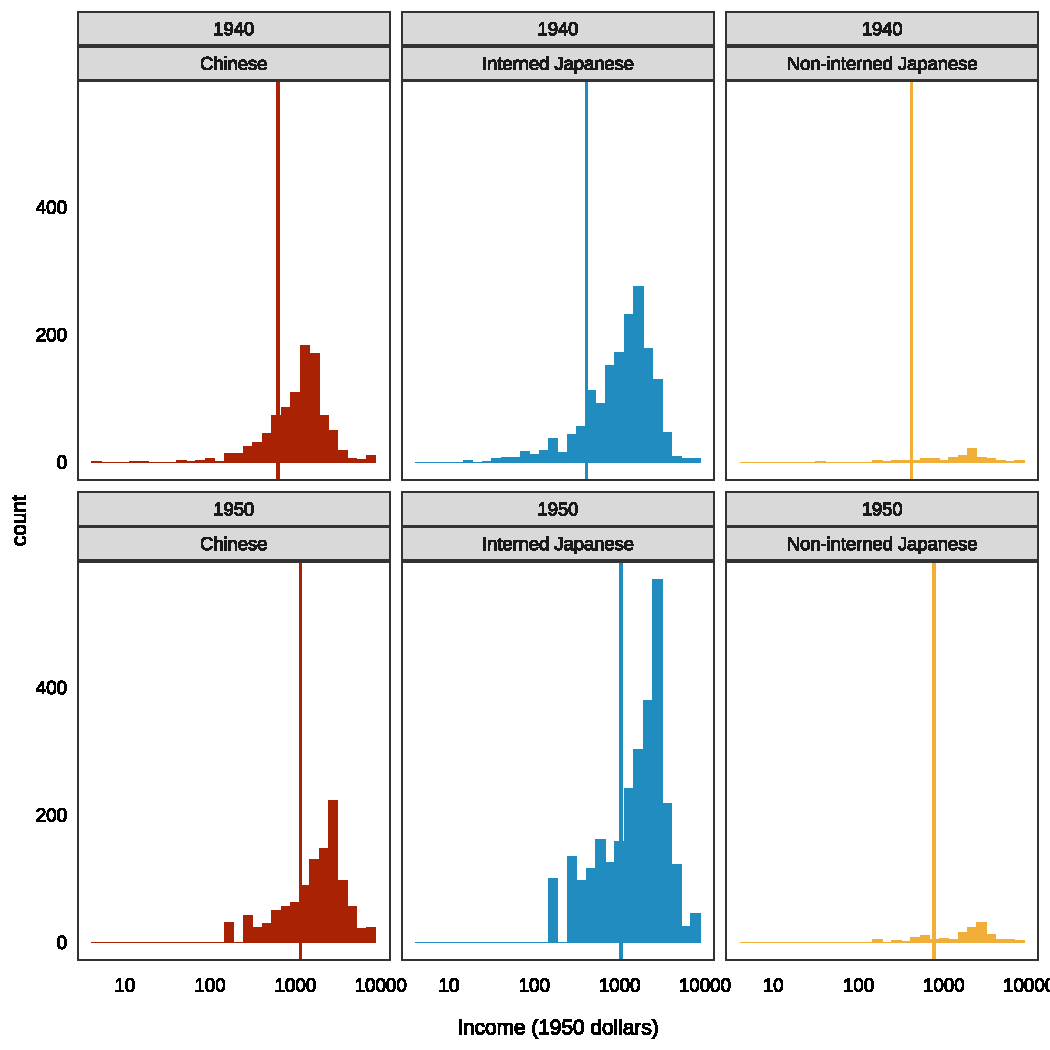
\includegraphics[width=\textwidth]{../figures/group-incwage-dist.pdf} \\
  \caption*{
    \footnotesize
    \emph{Note:}
    These histograms include all linked individuals
    from the main analysis sample.
    All Chinese individuals are treated as non-interned.
    `Interned Japanese' include all Japanese individuals
    with an estimated probability of greater than 0.75.
    `Non-interned Japanese' include all Japanese
    with an estimated probability equal to zero.
    Japanese with a probability between 0 and 0.75 are omitted
    in this figure.
    INCWAGE is the total earnings through wage employment
    from the year prior to each census year.
    Incomes in 1940 are adjusted for inflation to 1950 dollar amounts.
    }
\end{figure}

Figure \ref{fig:group-incwage-dist} shows the histograms of 
the natural log of INCWAGE,
the total earnings from wages and employment
(as opposed to earnings from self-employment, farming, etc.),
across the three different treatment groups
\footnote{see section \ref{eq:predint} for more details}
among the linked MLP sample.
The first column shows that Chinese in the control group did experience
real wage growth on average over these ten years.
The difference in the Chinese log income distribution shown here
translates into an average increase in wages of 84\%
(an increase from \$625 in 1940 to \$1151 in 1950).
Although interned Japanese and non-interned Japanese
both started with similarly low wages compared to the Chinese sample
(\$411 and \$419, respectively),
by 1950, the Japanese who were likely interned almost closed the gap
in average income compared to the Chinese (\$1037 vs \$1151),
while the non-interned Japanese still lagged behind
with an average wage of \$769.

In section \ref{sec:methods}, I describe the methodological tools I use
to argue that the convergence I observe between the likely internee group
and their outperformance relative their non-interned peers
captures a causal effect of internment and forced relocation
on the incomes earned in 1950.

\subsection{War Relocation Authority Records}

The WRA kept detailed records of the process of relocating and incarcerating 
the West Coast Japanese population.
I use the dataset from WRA Form 26: Evacuee Summary Data in the collection of 
Records About Japanese Americans Interned During World War II 
in the National Archives.
The original paper form from which this digitized version was coded 
included each internee's name, previous address in 1942, 
the assembly center and internment camp to which they were assigned,
their educational attainment, occupation, 
and demographics including sex, birth year, and birthplace.

Table \ref{tbl:wra_demog} reports a summary of the main demographic variables 
of internees compared to the full 1940 Japanese population.
Internees represented a large majority (86\%) 
of the Japanese population in the U.S. in 1940.
Internees were representative of the population in terms of their education, 
gender composition, and country of birth.
The 65\% of internees born in the U.S. 
represent the generation known as the ``Nisei'', 
or second generation after their parents, 
the ``Issei'', who make up most of the remaining 35\% of internees.
The average Issei was born in 1890, 
and would have been in their early fifties during internment,
while the average Nisei was born in 1927 
and would have been a teenager when interned.

Figure \ref{fig:internee-ages} shows the distribution 
of the age of internees at the time of the evacuation order in 1942.
This figure reveals that there was a large variation in the ages of internees 
and that the ten camps were fairly balanced in their age composition.
The most prominent age range in this figure is made up of young adults 
between the ages of 15 and 25. 

The WRA records also provide a mapping from the county of residence of all internees to the first camp they were placed.
Table \ref{tbl:cmp-cty} groups all internees by their previous address and their assigned camp.
The 20 largest counties with more than 1,000 interned residents are shown broken down by each of the ten camps.

Among the main internment counties are the major West Coast urban areas of Los Angeles, Seattle, Sacramento, San Francisco, and Portland.
However, there is also a large number of internees from more rural counties in California including Fresno, San Joaquin, Placer, and Tulare.
Interned Japanese came from a variety of backgrounds shown here by the range of urban and rural counties,
and also reflected in the range of occupations held by internees.

\begin{table}
  \caption{Demographics of Japanese Americans in 1940 Census and WRA records}
\centering
\begin{adjustbox}{width=\textwidth, center}
\begin{tblr}[         %% tabularray outer open
]                     %% tabularray outer close
{                     %% tabularray inner open
colspec={Q[]Q[]Q[]Q[]Q[]Q[]},
cell{2}{1}={}{halign=l,},
cell{2}{2}={}{halign=l,},
cell{3}{1}={}{halign=l,},
cell{3}{2}={}{halign=l,},
cell{4}{1}={}{halign=l,},
cell{4}{2}={}{halign=l,},
cell{5}{1}={}{halign=l,},
cell{5}{2}={}{halign=l,},
cell{6}{1}={}{halign=l,},
cell{6}{2}={}{halign=l,},
cell{7}{1}={}{halign=l,},
cell{7}{2}={}{halign=l,},
cell{8}{1}={}{halign=l,},
cell{8}{2}={}{halign=l,},
cell{9}{1}={}{halign=l,},
cell{9}{2}={}{halign=l,},
cell{10}{1}={}{halign=l,},
cell{10}{2}={}{halign=l,},
cell{11}{1}={}{halign=l,},
cell{11}{2}={}{halign=l,},
cell{12}{1}={}{halign=l,},
cell{12}{2}={}{halign=l,},
cell{13}{1}={}{halign=l,},
cell{13}{2}={}{halign=l,},
cell{14}{1}={}{halign=l,},
cell{14}{2}={}{halign=l,},
cell{1}{1}={}{halign=l, halign=c,},
cell{1}{2}={}{halign=l, halign=c,},
cell{2}{3}={}{halign=r,},
cell{2}{4}={}{halign=r,},
cell{2}{5}={}{halign=r,},
cell{2}{6}={}{halign=r,},
cell{3}{3}={}{halign=r,},
cell{3}{4}={}{halign=r,},
cell{3}{5}={}{halign=r,},
cell{3}{6}={}{halign=r,},
cell{4}{3}={}{halign=r,},
cell{4}{4}={}{halign=r,},
cell{4}{5}={}{halign=r,},
cell{4}{6}={}{halign=r,},
cell{5}{3}={}{halign=r,},
cell{5}{4}={}{halign=r,},
cell{5}{5}={}{halign=r,},
cell{5}{6}={}{halign=r,},
cell{6}{3}={}{halign=r,},
cell{6}{4}={}{halign=r,},
cell{6}{5}={}{halign=r,},
cell{6}{6}={}{halign=r,},
cell{7}{3}={}{halign=r,},
cell{7}{4}={}{halign=r,},
cell{7}{5}={}{halign=r,},
cell{7}{6}={}{halign=r,},
cell{8}{3}={}{halign=r,},
cell{8}{4}={}{halign=r,},
cell{8}{5}={}{halign=r,},
cell{8}{6}={}{halign=r,},
cell{9}{3}={}{halign=r,},
cell{9}{4}={}{halign=r,},
cell{9}{5}={}{halign=r,},
cell{9}{6}={}{halign=r,},
cell{10}{3}={}{halign=r,},
cell{10}{4}={}{halign=r,},
cell{10}{5}={}{halign=r,},
cell{10}{6}={}{halign=r,},
cell{11}{3}={}{halign=r,},
cell{11}{4}={}{halign=r,},
cell{11}{5}={}{halign=r,},
cell{11}{6}={}{halign=r,},
cell{12}{3}={}{halign=r,},
cell{12}{4}={}{halign=r,},
cell{12}{5}={}{halign=r,},
cell{12}{6}={}{halign=r,},
cell{13}{3}={}{halign=r,},
cell{13}{4}={}{halign=r,},
cell{13}{5}={}{halign=r,},
cell{13}{6}={}{halign=r,},
cell{14}{3}={}{halign=r,},
cell{14}{4}={}{halign=r,},
cell{14}{5}={}{halign=r,},
cell{14}{6}={}{halign=r,},
cell{1}{4}={}{halign=r, halign=c,},
cell{1}{6}={}{halign=r, halign=c,},
cell{1}{3}={c=2,}{halign=r, halign=c, halign=c,},
cell{1}{5}={c=2,}{halign=r, halign=c, halign=c,},
hline{5}={1,2,3,4,5,6}{solid, black, 0.05em},
}                     %% tabularray inner close
\toprule
&  & 1940 Census (N=126701) &  & Internees (N=109247) &  \\ \cmidrule[lr]{3-4}\cmidrule[lr]{5-6}
&    & Mean & Std. Dev. & Mean & Std. Dev. \\ \midrule %% TinyTableHeader
Birth Year &  & \num{1911.5} & \num{18.3} & \num{1912.5} & \num{18.9} \\
Years of Education &  & \num{7.9} & \num{4.3} & \num{8.0} & \num{4.4} \\
&  & N & Pct. & N & Pct. \\
Sex & Male & \num{71730} & \num{56.6} & \num{59480} & \num{54.4} \\
& Female & \num{54971} & \num{43.4} & \num{49755} & \num{45.5} \\
\hline
Country of Birth & Canada & \num{47} & \num{0.0} & \num{39} & \num{0.0} \\
& Japan & \num{47136} & \num{37.2} & \num{37941} & \num{34.7} \\
& Mexico & \num{29} & \num{0.0} & \num{10} & \num{0.0} \\
& South America & \num{0} & \num{0.0} & \num{3} & \num{0.0} \\
& United States & \num{79241} & \num{62.5} & \num{71200} & \num{65.2} \\
& NA & \num{248} & \num{0.2} & \num{54} & \num{0.0} \\
\bottomrule
\end{tblr}
\end{adjustbox}
\end{table}

